\documentclass[11pt]{report}

% Paquetes y configuraciones adicionales
\usepackage{graphicx}
\usepackage[export]{adjustbox}
\usepackage{caption}
\usepackage{float}
\usepackage{titlesec}
\usepackage{geometry}
\usepackage[hidelinks]{hyperref}
\usepackage{titling}
\usepackage{titlesec}
\usepackage{parskip}
\usepackage{wasysym}
\usepackage{tikzsymbols}
\usepackage{fancyvrb}
\usepackage{xurl}
\usepackage{hyperref}
\usepackage[spanish]{babel}
\usepackage{listings}
\usepackage{subcaption}
\usepackage{xcolor}
\usepackage{amssymb}

\newcommand{\subtitle}[1]{
  \posttitle{
    \par\end{center}
    \begin{center}\large#1\end{center}
    \vskip0.5em}
}

% Configura los márgenes
\geometry{
  left=2cm,   % Ajusta este valor al margen izquierdo deseado
  right=2cm,  % Ajusta este valor al margen derecho deseado
  top=3cm,
  bottom=3cm,
}

% Configuración de los títulos de las secciones
\titlespacing{\section}{0pt}{\parskip}{\parskip}
\titlespacing{\subsection}{0pt}{\parskip}{\parskip}
\titlespacing{\subsubsection}{0pt}{\parskip}{\parskip}

% Redefinir el formato de los capítulos y añadir un punto después del número
\makeatletter
\renewcommand{\@makechapterhead}[1]{%
  \vspace*{0\p@} % Ajusta este valor para el espaciado deseado antes del título del capítulo
  {\parindent \z@ \raggedright \normalfont
    \ifnum \c@secnumdepth >\m@ne
        \huge\bfseries \thechapter.\ % Añade un punto después del número
    \fi
    \interlinepenalty\@M
    #1\par\nobreak
    \vspace{10pt} % Ajusta este valor para el espacio deseado después del título del capítulo
  }}
\makeatother

% Configura para que cada \chapter no comience en una pagina nueva
\makeatletter
\renewcommand\chapter{\@startsection{chapter}{0}{\z@}%
    {-3.5ex \@plus -1ex \@minus -.2ex}%
    {2.3ex \@plus.2ex}%
    {\normalfont\Large\bfseries}}
\makeatother

% Configurar los colores para el código
\definecolor{codegreen}{rgb}{0,0.6,0}
\definecolor{codegray}{rgb}{0.5,0.5,0.5}
\definecolor{codepurple}{rgb}{0.58,0,0.82}
\definecolor{backcolour}{rgb}{0.95,0.95,0.92}

% Configurar el estilo para el código
\lstdefinestyle{mystyle}{
  backgroundcolor=\color{backcolour},   
  commentstyle=\color{codegreen},
  keywordstyle=\color{magenta},
  numberstyle=\tiny\color{codegray},
  stringstyle=\color{codepurple},
  basicstyle=\ttfamily\footnotesize,
  breakatwhitespace=false,         
  breaklines=true,                 
  captionpos=b,                    
  keepspaces=true,                 
  numbers=left,                    
  numbersep=5pt,                  
  showspaces=false,                
  showstringspaces=false,
  showtabs=false,                  
  tabsize=2
}

\begin{document}

\title{CANARY ISLANDS DATABASE}
\author{Samuel Martín Morales  \texttt{alu0101359526@ull.edu.es} \and Jorge Domínguez González  \texttt{alu0101330600@ull.edu.es} \and Cheuk Kelly Ng Pante \texttt{alu0101364544@ull.edu.es} }
\date{\today}

\maketitle

\chapter{Objetivos del Proyecto}
\begin{itemize}
    \item Diseñar e implementar una base de datos para gestionar información relacionada con las Islas Canarias.
    \item Crear una interfaz de programación de aplicaciones (API) que permita operaciones CRUD sobre la base de datos.
    \item Realizar consultas de prueba y demostrar el funcionamiento de la base de datos.
\end{itemize}

\chapter{Contexto y Requisitos}
\section{Entidades:}

\begin{itemize}
    \item \textbf{Islas:}
    \subitem - Atributos: ID (clave primaria), Nombre.
    
    \item \textbf{Distribución Poblacional:}
    \subitem - Atributos: ID (clave primaria), Nombre, Provincia, Capital, Municipio, Poblacion Isla.
    
    \item \textbf{Compañías:}
    \subitem - Atributos: ID (clave primaria), Nombre, Tipo, Sede (relacionada con Islas), Año Fundacion.
    
    \item \textbf{Sitio interes:}
    \subitem - Atributos: ID (clave primaria), Nombre, Isla, Municipio, Coordenadas, Foto.
    
    \item \textbf{Animales autóctonos:}
    \subitem - Atributos: ID (clave primaria), Nombre, Nombre Cientifico, Islas, Invasoras, Dieta, Foto.
    
\end{itemize}

\section{Relaciones:}

\begin{itemize}
    \item \textbf{Distribución Poblacional a Islas:}
    \subitem - Relacionada por la columna Nombre con la entidad Islas.
    
    \item \textbf{Compañías a Islas:}
    \subitem - Relacionada por la columna Sede con la entidad Islas.

    \item \textbf{Sitio interes a Islas:}
    \subitem - Relacionada por la columna Isla con la entidad Islas.

    \item \textbf{Animales autóctonos a Islas:}
    \subitem - Relacionada por la columna Islas con la entidad Islas.
\end{itemize}

\section{Consideraciones Adicionales:}

\begin{itemize}
    \item La relación entre las entidades Compañías y Islas se establece a través de la columna Sede, indicando la isla donde tienen su sede las compañías.
    \item La relación entre Sitios Interes y Islas se establece por la columna Isla, indicando en qué isla se encuentra el sitio de interés.
    \item La relación entre Animales autóctonos e Islas se establece por la columna Islas, indicando las islas a las que están asociados los animales autóctonos.
\end{itemize}

\section{Restricciones:}

\begin{itemize}
    \item La relación entre las entidades Compañías y Islas se establece a través de la columna Sede, indicando la isla donde tienen su sede las compañías.
    \item La relación entre Sitio interes y Islas se establece por la columna Isla, indicando en qué isla se encuentra el sitio de interés.
    \item La relación entre Animales autóctonos e Islas se establece por la columna Islas, indicando las islas a las que están asociados los animales autóctonos.
\end{itemize}
\chapter{Diseño Conceptual}

\section{Modelo Entidad-Relación}
\begin{figure}[H]
    \centering
    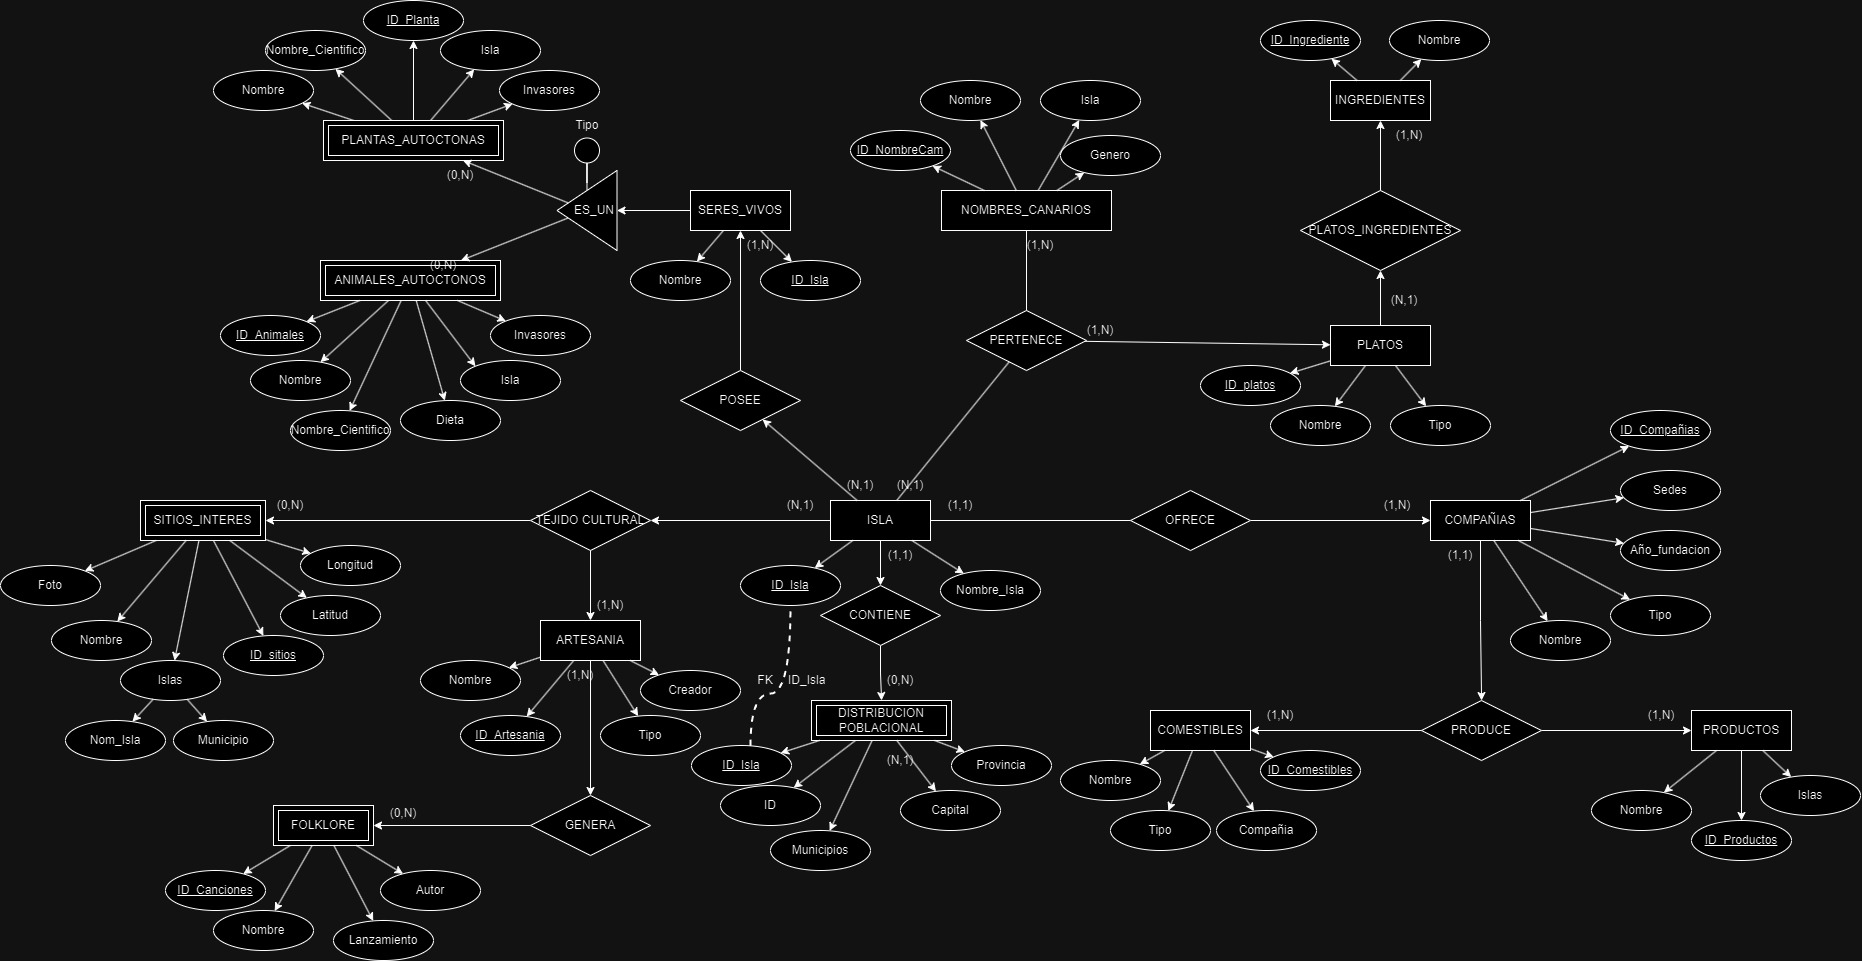
\includegraphics[width=0.9\textwidth]{../diagrams/ER-PF-ADBD.jpg}
    \caption{Modelo Entidad-Relación}
    \label{fig:modelo_er}
\end{figure}

\section{Modelo Relacional}
\begin{figure}[H]
    \centering
    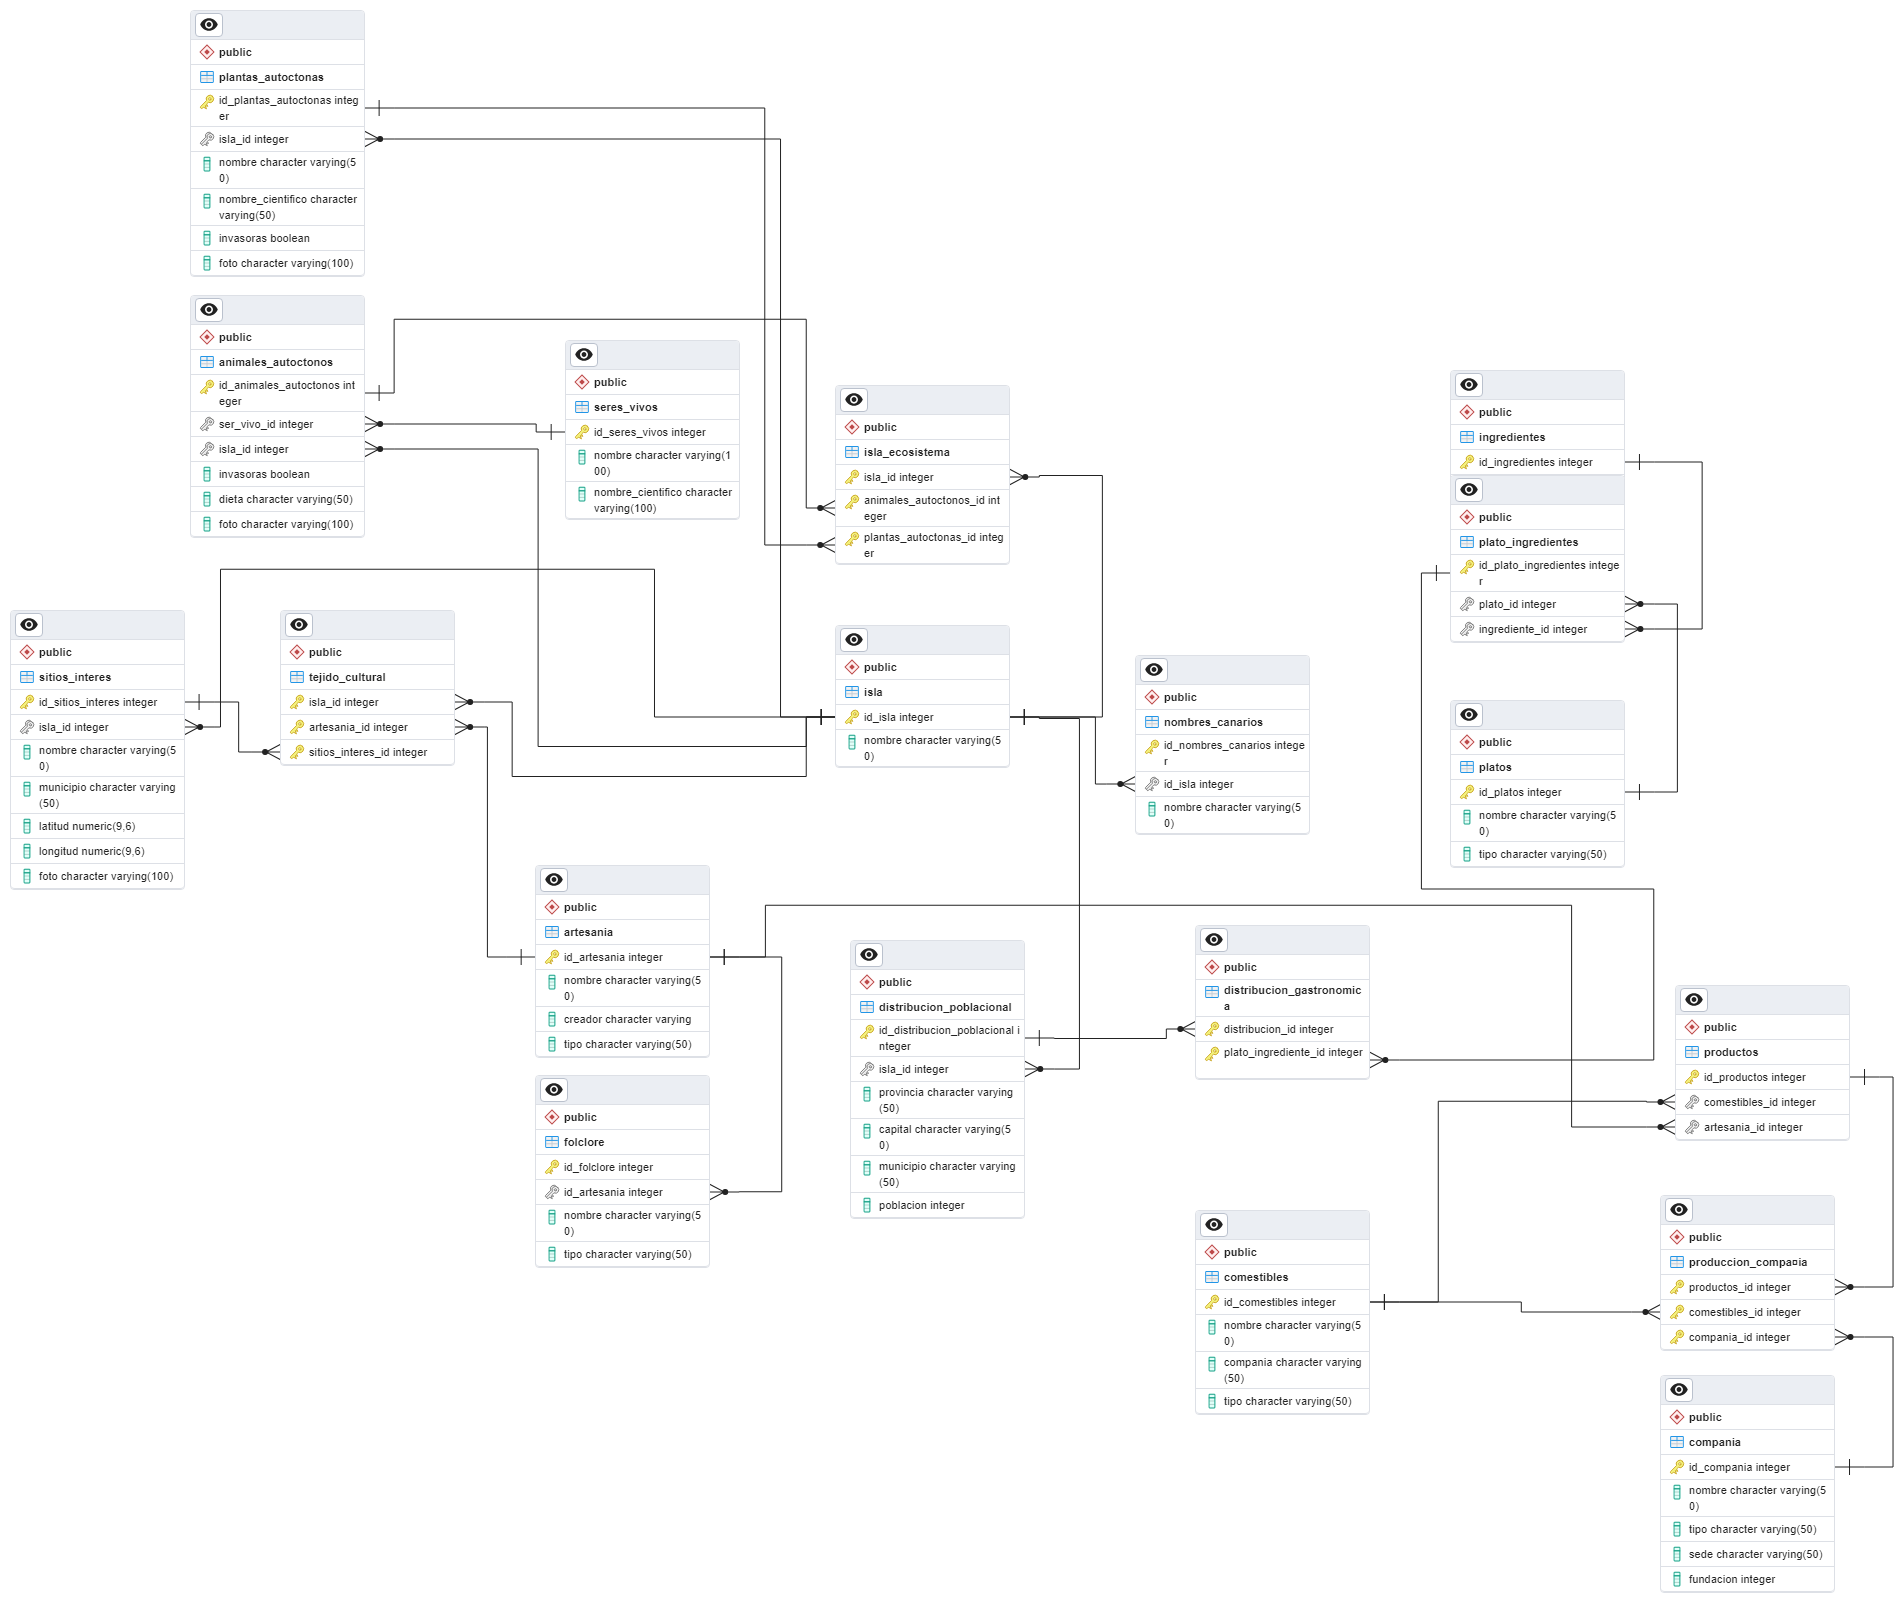
\includegraphics[width=0.9\textwidth]{../diagrams/RELACIONAL.jpg}
    \caption{Modelo Relacional}
    \label{fig:modelo_relacional}
\end{figure}

\section{Supuestos Semánticos}
Documentación que explique los supuestos semánticos y decisiones de diseño.

\chapter{Scripts SQL}

\chapter{Creación de la Base de Datos}
\begin{verbatim}
DROP DATABASE IF EXISTS islas_canarias;
CREATE DATABASE islas_canarias with TEMPLATE = template0 ENCODING = 'UTF8';

ALTER DATABASE islas_canarias OWNER TO postgres;

\connect islas_canarias

DROP SCHEMA IF EXISTS public CASCADE;
CREATE SCHEMA public;

ALTER SCHEMA public OWNER TO postgres;

SET default_tablespace = '';

SET default_table_access_method = heap;
\end{verbatim}

\chapter{Creación de Tablas y Datos de Muestra}
\begin{verbatim}
CREATE TABLE sitios_interes (
    id_sitios_interes SERIAL PRIMARY KEY,
    isla_id INTEGER NOT NULL,
    nombre VARCHAR(50) NOT NULL,
    municipio VARCHAR(50) NOT NULL,
    latitud DECIMAL(9,6) NOT NULL,
    longitud DECIMAL(9,6) NOT NULL,
    foto VARCHAR(100) NOT NULL,
    CONSTRAINT sitios_interes_isla_fkey
        FOREIGN KEY (isla_id)
        REFERENCES isla  (id_isla) ON DELETE CASCADE
);
\end{verbatim}

\chapter{Inclusión de Datos en las Tablas}
\begin{verbatim}
-- -- Inclusión de datos en la tabla de isla_ecosistema
ALTER TABLE isla_ecosistema
ALTER COLUMN plantas_autoctonas_id DROP NOT NULL,
ALTER COLUMN animales_autoctonos_id DROP NOT NULL;

TRUNCATE TABLE isla_ecosistema;

INSERT INTO isla_ecosistema(isla_id, seres_vivos_id, animales_autoctonos_id, plantas_autoctonas_id)
SELECT isla_id, ser_vivo_id, id_animales_autoctonos, NULL
FROM animales_autoctonos;

INSERT INTO isla_ecosistema(isla_id, seres_vivos_id, animales_autoctonos_id, plantas_autoctonas_id)
SELECT isla_id, ser_vivo_id, NULL, id_plantas_autoctonas
FROM plantas_autoctonas;
\end{verbatim}

\chapter{Implementación de Triggers}
\begin{verbatim}
-- Si se añade una nueva tupla dentro de la tabla de animales_autoctonos, se añadirá una nueva tupla en la tabla de isla_ecosistema
CREATE OR REPLACE FUNCTION insertar_animal_autoctono() RETURNS TRIGGER AS $$
BEGIN
    INSERT INTO isla_ecosistema(isla_id, seres_vivos_id, animales_autoctonos_id, plantas_autoctonas_id)
    VALUES (NEW.isla_id, NEW.ser_vivo_id, NEW.id_animales_autoctonos, NULL);
    RETURN NEW;
END;
$$ LANGUAGE plpgsql;

CREATE TRIGGER insertar_animal_autoctono
AFTER INSERT ON animales_autoctonos
FOR EACH ROW
EXECUTE PROCEDURE insertar_animal_autoctono();
\end{verbatim}

\chapter{Consultas de Ejemplo}

\section{Consultas SQL}
Ejemplos de consultas que demuestren el funcionamiento de la base de datos.

\chapter{Implementación de API con Flask}

\section{API REST}
Desarrollo de una API mediante Flask para realizar operaciones CRUD.

\chapter{Entrega}

\section{Repositorio en GitHub}
Enlace al Repositorio: \url{https://github.com/feichay10/Proyecto-Final-ADBD/tree/main}

\section{Imágenes Adjuntas}
Modelo Entidad-Relación, Grafo Relacional y capturas de consultas y operaciones en las tablas.

\chapter{Bibliografía}
\begin{thebibliography}{99}
    \bibitem{1} \url{https://www.canaryislands.org/}

\end{thebibliography}

\end{document}
